\chapter{Besonderheiten der Dynamischen Wegfindung}

\section{Kommunikation}
	\label{Kommunikation}
	Eine Grundvoraussetzung für jegliche Art von Dynamik ist das Wissen über die eigene Umgebung. Es ist nicht möglich, dynamisch auf Ereignisse zu reagieren, wenn Daten über die Umgebung seit der initialen Wegberechnung nicht aktualisiert wurden. Aus diesem Grund ist Kommunikation als Mittel der Informationsbeschaffung essentiell. Da das Anwenderprogramm modularisiert und in Schichten aufgeteilt wurde, ist ein Datenaustausch unabdingbar. 
	\\[4pt]
	Da das Projekt von zwei Personen bearbeitet und die Kommunikation zwischen beiden Teilschichten separat entwickelt wurde, kann die Kommunikationsschicht in zwei getrennte Unterschichten aufgeteilt werden. Jede dieser Teilschichten regelt die Schnittstelle zu der zugehörigen Schicht. Aus diesem Grund wird in folgenden Abschnitt vor allem die Kommunikation aus Sicht der Wegfindung beschrieben. Beide Unterschichten wurden aber aufeinander abgestimmt und sind im Kern identisch und haben nur unterschiedliche Verwendungsarten und Implementierungen.
	\\[4pt]
	Wie bereits erwähnt, erfüllt die Kommunikationsschicht vor allem zwei Anforderungen. Die erste Anforderung ist der Datenaustausch zwischen den Schichten des Anwenderprogramms eines einzelnen \ac{FTF}. Da in der vorliegenden Realisierung der Anlage sowohl die Wegfindung als auch die Fahrzeugsteuerung auf der selben Steuerung ausgeführt werden, wurde diese Kommunikationsart als "`Interne Kommunikation"' bezeichnet. Im Gegensatz hierzu wurde der Austausch von Informationen zwischen anderen Fahrzeugen "`Externe Kommunikation"' genannt. Abbildung \ref{Kommunikationsschicht Gliederung} zeigt das Zusammenspiel der einzelnen Teilschichten. Es ist grundsätzlich möglich, beide Arten der Kommunikation gemeinsam zu implementieren. Da aber für den Datenaustausch innerhalb der \ac{SPS} das externe Netz nicht unnötig belastet werden muss, wurde entschieden die beiden Arten von Kommunikation aufzutrennen. Dies hat den weiteren Vorteil das bei internem Datenaustausch die Daten schneller für die jeweils andere Schicht verfügbar sind, als dies beispielsweise über eine drahtlose Verbindung der Fall wäre.
	
	\begin{figure}[h]
		\centering
		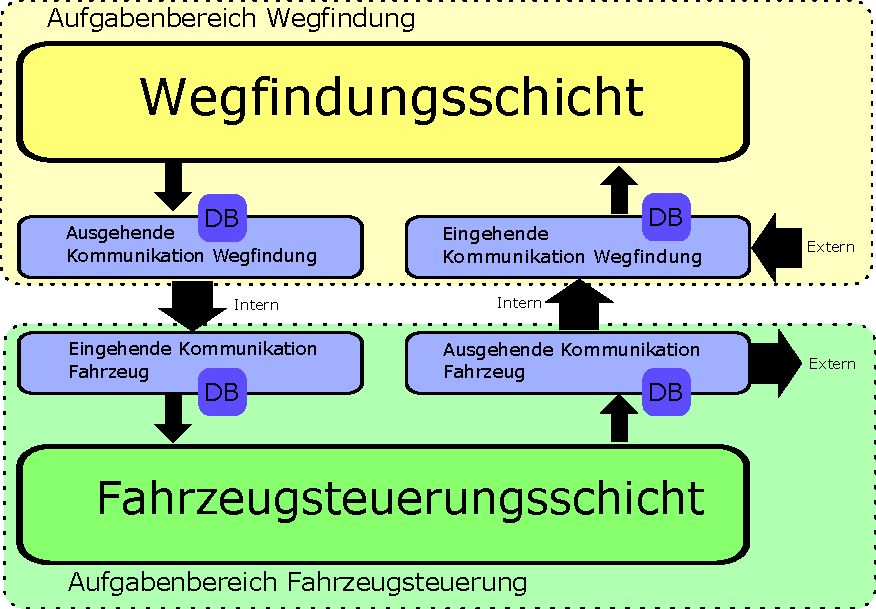
\includegraphics[scale=0.9]{/Bilder/KommunikationSchichtenPDF}
		\vspace{0.2cm}
		\caption{Feinuntergliederung der Kommunikationsschicht.}\label{Kommunikationsschicht Gliederung}
	\end{figure}
	
	\subsection{Schnittstelle zur Kommunikationsschicht}
		
		Beide Arten der Kommunikation besitzen die selbe strukturellen Anbindung an die zugehörige Programmschicht. Für die eingehende und ausgehende Kommunikation existiert jeweils ein Schnittstellen-\ac{DB}. Beide \ac{DB}s besitzen den folgenden grundsätzlichen Aufbau:
		
		\begin{itemize}
			\item Speicherplatz für Daten zur internen Kommunikation.
			\item Speicherplatz für Daten zur externen Kommunikation.
			\item Signalisierungsbits zum Erkennen oder Anstoßen der Kommunikation.
		\end{itemize}
		
		Am Beispiel der Wegfindungsschicht bedeutet dies, dass der Schnittstellen-\ac{DB} für die ausgehende Kommunikation aus einem Datentyp für den internen Datenaustausch besteht,der die in Abschnitt \ref{Routengeneration} beschriebenen Routeninformationen enthält. Der externe Datenaustausch mit anderen Fahrzeugen wird mit einem Byte-Array konstanter Größe realisiert. Für die Wegfindung kommt als einziger möglicher Partner für eine ausgehenden Verbindung jedoch nur die korrespondierende Fahrzeugsteuerung  in Frage. Aus diesem Grund wird das Byte-Array bei der Implementierung der Wegfindungs- und Fahrzeugsteuerungsschicht auf der gleichen Steuerung  im Schnittstellen-\ac{DB} für die ausgehende Kommunikation hier nicht benötigt. Stattdessen wird der intern verwendete Routendatentyp übertragen, da bei dem internen Kopiervorgang eine Aufspaltung in die einzelnen Bytes nicht benötigt wird. Das vorhandene Signalisierungsbit, in Abbildung \ref{InterfaceDB} mit "`send"' bezeichnet, gibt eine Sendeanforderung für die Route aus der Wegfindungsschicht an die Kommunikationsunterschicht der Wegfindung weiter. Die entsprechenden Bausteine reagieren auf diese Anforderung und stoßen die Übertragung an.
		
		\begin{figure}[h]
			\centering
			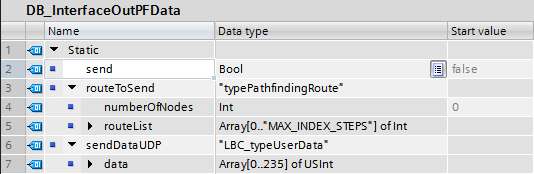
\includegraphics[scale=0.8]{/Bilder/TIA_InterfaceDBAusgehend}
			\vspace{0.2cm}
			\caption{Aufbau des Schnittstellen-\ac{DB} für ausgehende Kommunikationsverbindungen.}\label{InterfaceDB}
		\end{figure}

		Der Schnittstellen-DB für die eingehende Kommunikation besitzt analog zum Ausgehenden zwei Datenbereiche für interne und externe Kommunikation, wobei hier beide als Byte-Arrays realisiert sind. Im Unterschied zum vorherigen \ac{DB} enthält dieser zwei getrennte Signalisierungsmerker für intern und extern erhaltene Daten. Der Grund hierfür ist die zeitliche Staffelung der beiden Kommunikationsarten, die in Abschnitt \ref{Anpassung Kommunikation} näher erläutert wird.
		
	\subsection{Interne Kommunikation}
		\label{Interne Kommunikation}
		Die Interne Kommunikation besteht aus Sicht der Wegfindung vor allem aus dem Empfangen von Positionsdaten der zugeordneten Fahrzeugsteuerung und Senden der berechneten Routen an Selbige. Die Fahrzeugsteuerung erkennt durch den vorgelagerten \ac{RFID}-Sensor den voraus liegenden Knoten und teilt diesen der Wegfindung mit. Da sich beide Schichten auf der gleichen Steuerung befinden besteht hier die interne Kommunikation der Einfachheit halber nur aus dem Kopieren der Positionsdaten aus dem ausgehenden Schnittstellen-\ac{DB} der Fahrzeugsteuerung in den entsprechenden Speicherplatz im eingehenden \ac{DB} der Wegfindungsschicht. Um die Wegfindungsschicht über die neuen Daten in Kenntnis zu setzen, wird das interne Signalisierungsbit im eingehenden Schnittstellen-\ac{DB} der Wegfindung einen Zyklus lang gesetzt.
		\\[4pt]
		Die Positionsdaten haben bei der Implementierung mittels Byte-Array den folgenden Aufbau:\\
		
		\begin{table}[h]
			\begin{tabular}{| c | l |}
				\hline
				\textbf{Arrayindex} & \textbf{Bedeutung} \\ \hline \hline
				0 & ID des sendenden Fahrzeugs. \\ \hline
				1 & ID des erkannten aktuellen (\ac{RFID}-)Knotens. \\ \hline
				2 & ID des nächsten Knotens entlang der aktuellen Route. \\
				\hline
			\end{tabular}\\
			\caption{Aufbau des Arrays zur Übertragung von Positionsdaten.}
		\end{table}
		Die ID des sendenden Fahrzeugs wird für die interne Kommunikation nur dann benötigt, wenn sich die Wegfindung nicht auf der selben Steuerung wie die Fahrzeugsteuerung befindet. Durch die ID des aktuellen Knotens wird die bevorstehende Kreuzung identifiziert. Anhand des Knotens an Index 2, zu dem an der bevorstehenden Kreuzung nach der derzeitigen Route abgebogen wird, kann die Teilstrecke\footnote{Verbindungskante zwischen aktuellem und nächstem Knoten.} bestimmt werden, die das \ac{FTF} voraussichtlich als nächstes befahren wird.Abbildung \ref{Identifikation Teilstrecke} zeigt, wie aus den Positionsdaten die nächste Teilstrecke eines Fahrzeugs bestimmt werden kann. Diese Angabe ist vor allem für die Kollisionsvermeidung in Abschnitt \ref{Kollisionsvermeidung} von Bedeutung. Stimmen die beiden KnotenIDs der Positionsdaten überein, so bedeutet dies, dass der Zielknoten einer Teilroute erreicht wurde. Gemäß Abschnitt \ref{Simulation Station} wird hiermit die Simulation der Bearbeitungsdauer gestartet und die Berechnung der nächsten Teilroute angestoßen.
		
		\begin{figure}[h]
			\centering
			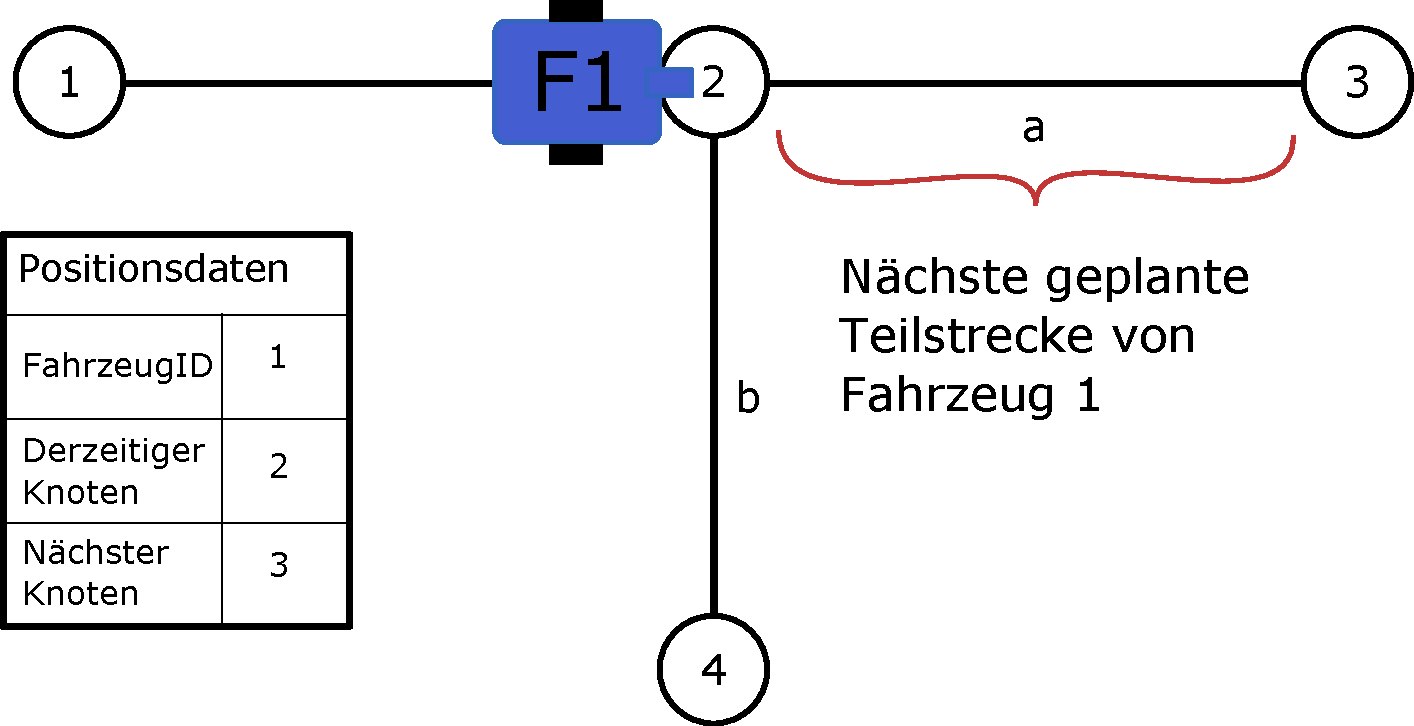
\includegraphics[scale=0.6]{/Bilder/IdentifikationTeilstreckePDF}
			\vspace{0.2cm}
			\caption{Ermittlung der nächsten geplanten Teilstrecke eines Fahrzeugs anhand der erhaltenen Positionsdaten.}\label{Identifikation Teilstrecke}
		\end{figure}
		
		Um eine berechnete Teilroute an die Fahrzeugsteuerung zu übersenden, wird diese zunächst im ausgehenden Schnittstellen-\ac{DB} im Speicherbereich für die Route abgelegt. Durch Setzen des Signalmerkers wird ein Kopiervorgang, analog zu dem beim Erhalten der Positionsdaten, gestartet und nach Abschluss der Übertragung das Signalisierungsbit des eingehenden Schnittstellen-{DB}s der Fahrzeugsteuerung gesetzt. Dies signalisiert, dass dem Fahrzeug eine neue Teilroute zur Verfügung gestellt wurde. Dies bedeutet eigentlich, das die internen Kommunikationsbausteine der beiden Unterschichten in diesem Fall nicht unabhängig voneinander sind, da sie den eingehenden \ac{DB} der jeweils anderen Schicht kennen müssen, um die Daten dort abzulegen. Dies wurde aufgrund der einfacheren Implementierung jedoch in Kauf genommen und bedeutet nicht, das dies auch bei Verwendung anderer Kommunikationsbausteine\footnote{beispielsweise Bausteine für Kommunikation über \ac{TCP}.} der Fall ist.
				
	\subsection{Externe Kommunikation}
		\label{Externe Kommunikation}
		Mittels der externen Kommunikation, werden die eigenen Positionsdaten den anderen Fahrzeugen in der gleichen Anlage mitgeteilt. Da die Übermittlung von Positionsdaten eine Aufgabe der Fahrzeugsteuerung ist, werden von der Wegfindungsschicht nur Daten empfangen und keine versandt. Aufgrund der Tatsache, dass die Fahrzeuge mobil sein müssen, wurde zur Datenübertragung an andere Fahrzeuge eine drahtlose Verbindung ausgewählt. Hierfür verfügt jedes \ac{FTF} über sein eigenes \acs{WLAN}-Client-Modul. Zudem existiert in der Anlage an zentraler Stelle ein \acs{WLAN}-Access-Point der sicherstellt, das Übertragungen alle Fahrzeugen innerhalb der Anlage erreichen. Als Übertragungsprotokoll wurde das \ac{UDP} gewählt, da im Rahmen dieses Protokolls ungerichtete Verbindungen aufgebaut werden können. Dies hat den Vorteil, das mittels einer ungerichteten Verbindung die Broadcast-Adresse des Netzwerksegments als Verbindungspartner projektiert werden kann, was bei \ac{TCP} nicht der Fall ist.
		\\[4pt]
		Diese Broadcast-Adresse ist eine reservierte Spezialadresse innerhalb eines Subnetzes, welche die Eigenschaft hat, das sie von allen Teilnehmern im gleichen Netzwerkabschnitt empfangen und ausgewertet wird. Diese Eigenschaft wird im vorliegenden Fall ausgenutzt, um Informationen an alle Netzwerkteilnehmer weiter zu leiten, ohne die spezifischen Netzwerkadressen der Teilnehmer kennen zu müssen. Zudem wird nur eine einzige Verbindung pro Positionsübertragung benötigt. Dies hat den Vorteil, dass es gleich ist, welche anderen \ac{FTF} sich zu einem bestimmten Zeitpunkt in der Anlage befinden. Solange die Fahrzeuge mit dem gleichen Netzsegment verbunden sind, können sie Daten von anderen Fahrzeugen empfangen und eigene Positionsdaten senden. Das gleiche gilt auch für Überwachungs- und Visualisierungssysteme, die einfach in das gleiche Subnetz eingehängt werden können um den Netzverkehr abzuhören, ohne den Betrieb der Anlage zu behindern.
		\\
		\textbf{insert network graphic here}
		\\
		Über diese Verbindung übermittelt jedes Fahrzeug ähnliche\footnote{die Unterschiede sind in Abschnitt \ref{Anpassung Kommunikation} beschrieben} Informationen wie bei der internen Kommunikation an das Netz. Die somit erhaltenen Positionsdaten der anderen Fahrzeuge werden in der in Kapitel \ref{Bearbeitungsreihenfolge} eingeführten Liste der erfassten Fahrzeugdaten gesichert. Diese enthält somit Informationen über die zuletzt empfangene Position eines anderen Fahrzeugs. Sollte ein Fahrzeug den Sendevorgang eines anderen \ac{FTF} nicht mitbekommen, so wird spätestens beim nächsten Sendevorgang die Position aktualisiert.
		
	\subsection{Vorteile der Modularität}
		
		Der modulare Aufbau des Anwenderprogramms hat nicht nur den Vorteil, dass die Wegfindungsschicht auf eine zentrale Steuereinheit ausgelagert werden kann. Vor allem bei der Kommunikation können durch die Modularisierung verschiedene Kommunikationsarten einfach und schnell gegeneinander ausgetauscht werden. Im Verlauf der Entwicklung des Anlagenmodells wurden verschiedene Übertragungsarten auf ihre Vor- und Nachteile hin untersucht.
		Folgende Kommunikationsmöglichkeiten wurden getestet:
		
		\begin{itemize}
			\item \textbf{\ac{UDP}:} 
				\begin{itemize}
					\item \textbf{Vorteil}: Gleichzeitige Adressierung aller Fahrzeuge ohne Wissen derer Adressen möglich.
					\item \textbf{Nachteil}: Ungerichtete Verbindung gibt keine Informationen über den Erhalt der Daten zurück.
				\end{itemize}
			\item \textbf{\acs{TCP}:}
				\begin{itemize}
					\item \textbf{Vorteil}: Durch Verbindungsüberwachung werden Daten bei Verlust automatisch neu versendet. Geeignet für gesicherte Übertragung von Routen.
					\item \textbf{Nachteil}: Eigene dedizierte Verbindung nötig zu jedem anderen Netzteilnehmer. Auf den kleinen S7-1200er Steuerungen aufgrund der auf acht beschränkten Anzahl gleichzeitige programmierter Verbindungen\cite{S7-1200} nur begrenzt einsetzbar, da hiermit die Anzahl der Fahrzeuge beschränkt wird oder eine zentrale Kommunikationseinheit für die Verteilung der Daten an die anderen Fahrzeuge zuständig sein muss.
				\end{itemize}
			\item \textbf{\ac{UDP}-Broadcast Master-Slave \cite{MasterSlaveUDP}:}
				\begin{itemize}
					\item \textbf{Vorteil}: Erreichbare Teilnehmer werden detektiert erfolgreiche Übertragung wird bestätigt.
					\item \textbf{Nachteil}: Nur die Masterstation kann senden. Wechseln des Masters dauert mit zirka 200ms verhältnismäßig lange und ist deshalb nur für wenige Teilnehmer realisierbar. 
				\end{itemize}
			\item \textbf{Internes Kopieren:}
			\begin{itemize}
				\item \textbf{Vorteil}: Schnelles, fehlersicheres Verfahren.
				\item \textbf{Nachteil}: Nur für Kommunikation auf gleicher Steuerung einsetzbar. Bricht streng genommen die Modularität, da Wissen über den Verbindungspartner vorhanden sein muss.
			\end{itemize}
		\end{itemize}
		
		Durch die Unabhängigkeit der Schichten kann die Funktionalität der Modellanlage innerhalb gewisser Grenzen an die gegebenen Anforderungen angepasst werden, ohne die Funktionalität anderer Schichten zu beeinträchtigen.

\section{Algorithmische Kollisionsvermeidung}
	\label{Kollisionsvermeidung}
		
	Wenn sich mehrere \ac{FTF} zur gleichen Zeit in der Anlage befinden, muss für eine funktionierende Anlage verhindert werden, das sich die Wege dieser Fahrzeuge kreuzen. Es muss somit verhindert werden, dass zwei Fahrzeuge zeitgleich den selben Streckenabschnitt befahren.  Die Fahrzeuge verfügen an der Vorderseite über einen Reflex-Lichtschranken-Sensor zur Kollisionserkennung. Dieser hält das \ac{FTF} bei Erkennung eines Hindernisses an, indem die Motoren abgeschaltet werden. Verschwindet das Hindernis, setzt das Fahrzeug selbstständig die aktuelle Route fort. Da dieser Sensor bei der Erkennung eines voran fahrenden Fahrzeugs ein mögliches Auffahren verhindert, ist es somit kein Problem, wenn beide Fahrzeuge auf dem gleichen Streckenabschnitt hintereinander in die gleiche Richtung fahren. Da ein \ac{FTF} jedoch nur an Knotenpunkten die Richtung ändern kann, muss unbedingt verhindert werden, dass sich zwei Fahrzeuge auf dem gleichen Streckenabschnitt entgegen kommen. Abbildung \ref{FTS Seite Sensoren} zeigt die Anordnung der relevanten Sensoren am Fahrzeug. Bei Einstellung einer großen Reichweite des Kollisionssensors  würden sich die Fahrzeuge gegenseitig erkennen und permanent stehen bleiben. Sind die Kollisionssensoren jedoch kurz eingestellt, stoßen die tiefliegenden \ac{RFID}-Ausleger zusammen, da sie zu weit unten angebracht sind, um von dem Sensoren erkannt zu werden. 
	
	\begin{figure}
		\centering
		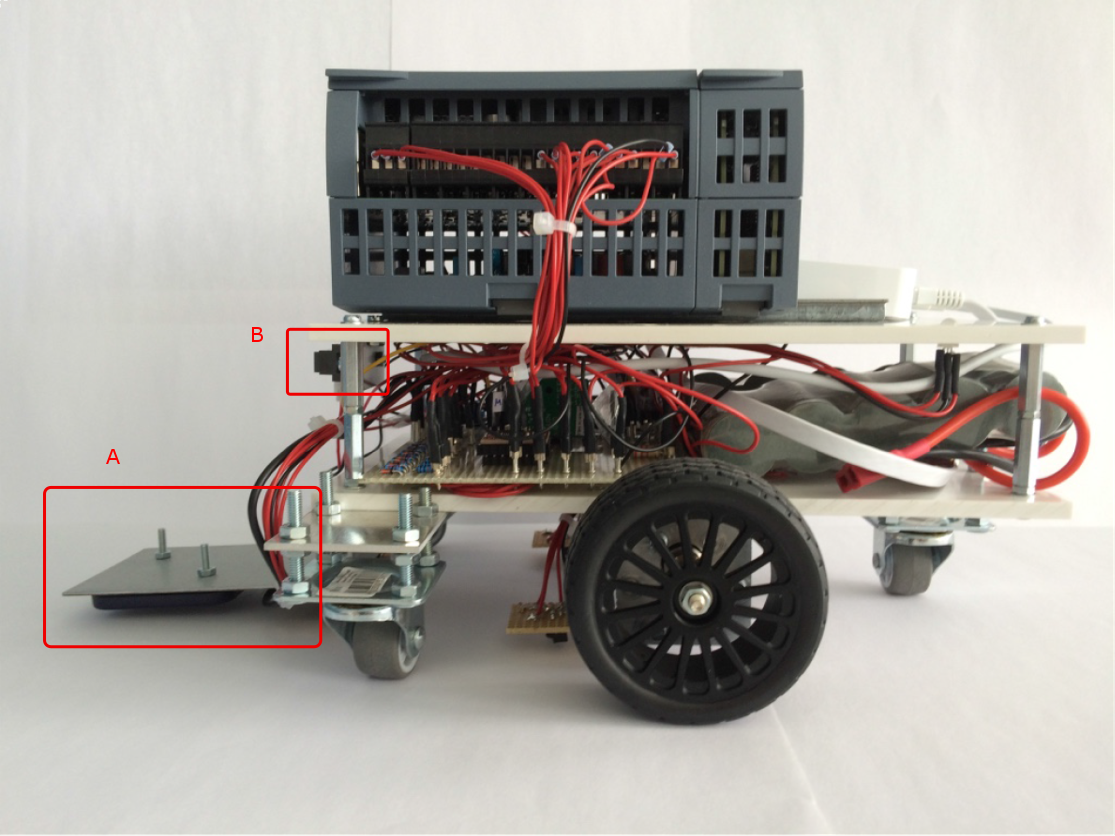
\includegraphics[scale= 0.5, clip, trim = 0mm 50mm 150mm 80mm]{/Bilder/FTS_Seitenansicht}
		\vspace{0.2cm}
		\caption{Seitenansicht des \ac{FTF}. A ist der tiefliegende \ac{RFID}-Sensorausleger, B der höher befestigte optische Kollisionssensor.} \label{FTS Seite Sensoren}
	\end{figure}
	
	\subsection{Generelle Vorgehensweise bei Kooperativen Wegfindungsalgorithmen}
		\label{Coop Pathfinding}
		Um die Vorgehensweise der algorithmischen Kollisionsvermeidung klar darstellen zu können, ist es von Vorteil, zunächst die Grundzüge der kooperativen Wegfindung zu erläutern. Vor allem in Computersimulationen und Computerspielen werden häufig Algorithmen verwendet, welche die Bewegungen mehrerer Einheiten koordinieren und aufeinander abstimmen. 
		\\[4pt]
		Um sicher zu stellen, dass Einheiten einen optimalen Weg nehmen, ohne sich gegenseitig zu behindern, ist es nötig, die Wege aller beteiligten Akteure zu kennen und diese in den Wegfindungsalgorithmus mit einfließen zu lassen. Die Berechnung des Weges stützt sich hierbei beispielsweise auf eine dreidimensionale Matrix, bei der die ersten beiden Dimensionen die Topologie und die dritte Dimension die Zeit darstellen. Da sich Einheiten getaktet fortbewegen kann somit jeder Einheit innerhalb dieser Matrix zu jedem Zeitpunkt ein bestimmter Index zugeordnet werden \cite{Silver2005}. Abbildung \ref{SpaceTimeMatrix} zeigt eine solche Zuordnung anhand einer einfachen Topologie. Diese Vorgehensweise kann verglichen werden mit der Reservierung eines bestimmten Knotenpunktes zu einem gegebenen Zeitpunkt, zu dem dieser Knoten für andere Einheiten blockiert ist \cite{Erdmann1986}. Andere Einheiten planen ihre Routen unter Berücksichtigung bereits bestehender Reservierungen.
		
		\begin{figure}[h]
			\centering
			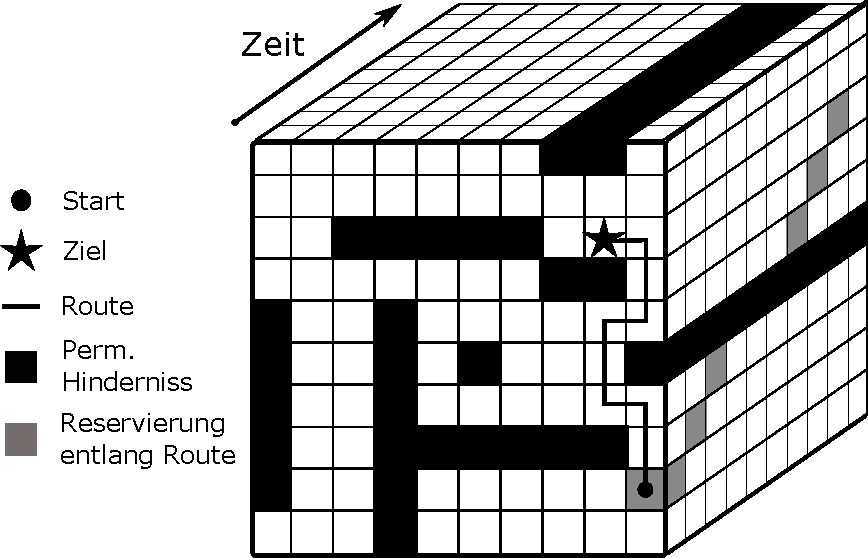
\includegraphics[scale=0.8]{/Bilder/SpaceTimeMatrixPDF}
			\vspace{0.2cm}
			\caption{Dreidimensionale Matrix mit Reservierung von Knoten  zu bestimmten Zeitpunkten entlang einer Route. Angelehnt an \cite{Silver2005}.}\label{SpaceTimeMatrix}
		\end{figure}
		
		In der hier realisierten Modellanlage ist diese Vorgehensweise jedoch nur begrenzt anwendbar. Da die Wegberechnung auf die einzelnen Fahrzeuge verteilt ist und nicht zentral gesammelt durchgeführt wird, müsste jedes Fahrzeug immer seine komplette Teilroute allen Anderen mitteilen. Dies ist theoretisch möglich, würde aber die Kommunikationslast deutlich erhöhen somit die Skalierbarkeit der Anlage verschlechtern.
		\\[4pt]
		Ein weiterer Unterschied ist, dass im vorliegenden Anwendungsfall nicht die Graphenknoten reserviert werden müssten, sondern die Verbindungskanten, da diese die blockierten Streckenabschnitte darstellen. Da die Anlage um einiges mehr Kanten besitzt als Knoten, ist es aufgrund der Speicherbeschränkungen der leistungsschwächeren Steuerungen nicht möglich, Matrizen mit einer hohen Zeitgranularität zu verwenden.

	\subsection{Problem des Zeitlichen Indeterminismus}
		\label{Zeitproblem}
		Das größte Hindernis bei der Implementierung eines puren kooperativen Wegfindungsalgorithmus ist jedoch das Taktungsproblem. Anders als bei den in Abschnitt \ref{Coop Pathfinding} vorgestellten Anwendungsgebieten bewegen sich die einzelnen Fahrzeuge nicht in konstanter Zeit von einem Streckenabschnitt zum Nächsten. Systembedingt haben nicht alle Teilstrecken die gleiche Länge. Zudem schwankt die Fahrgeschwindigkeit einer einzelnen \ac{FTF} je nach Ladezustand der Akkus sehr stark. Dies macht Vorhersagen über die Position eines Fahrzeugs sehr ungenau, je weiter man in der Zeit vorausschaut.
		\\[4pt]
		Eine Möglichkeit, die Vorhersagen zu verbessern wäre, anhand von Zeitmessungen Werte für die Belegdauer von Teilstrecken zu bestimmen und diese dann als Basis für die Vorhersagen zu benutzen. Dies birgt jedoch das Problem, dass das Verhältnis von Fahrtzeit auf einer Strecke zu der Zeit die benötigt wird um an einem Knoten ab zu biegen nicht vernachlässigbar ist. Somit müssten für jede einzelne Verbindungsstrecke mehrere Messungen gemacht werden, die alle Abbiegemöglichkeiten beinhalten. Bei der Vorhersage muss in diesem Fall aus den verschiedenen Messungen diejenige ausgewählt werden, die für diese Kombination aus Teilstrecken die Richtige ist. Dies erhöht den ohnehin bereits hohen Speicherbedarf der Wegfindung. Zudem würde hierbei immer noch der Ladezustand der Akkus nicht mit berücksichtigt werden, der wie bereits erwähnt zu starken Geschwindigkeitsunterschieden führen kann.
		\\[4pt]
		Bei genauerer Betrachtung lässt sich aussagen, dass als brauchbare Vorhersage für die Position nur die Beschränkung auf die unmittelbare Zukunft sinnvoll ist. Dies bedeutet das beim erreichen eines Entscheidungsknotens nur mit Sicherheit gesagt werden kann, auf welcher der vier möglichen Verbindungsstrecken sich das Fahrzeug als nächstes befinden wird.\textbf{insert clarification graphic here} Bei einem dynamischen System kann es vorkommen, das die geplante Route am nächsten Knoten bereits wieder verworfen wird und somit etwaige Vorhersagen über die erste Verbindungskante hinaus ohnehin nicht mehr gültig, sondern nur noch eine von vier möglichen Teilrouten sind, wie Abbildung \ref{Einstufig} zeigt. Nur über grüne Teilstrecken kann bei Erreichen des Knoten "`1"' mit Gewissheit eine Aussage über deren Belegungszustand gemacht werden.
		
		\begin{figure}[h]
			\centering
			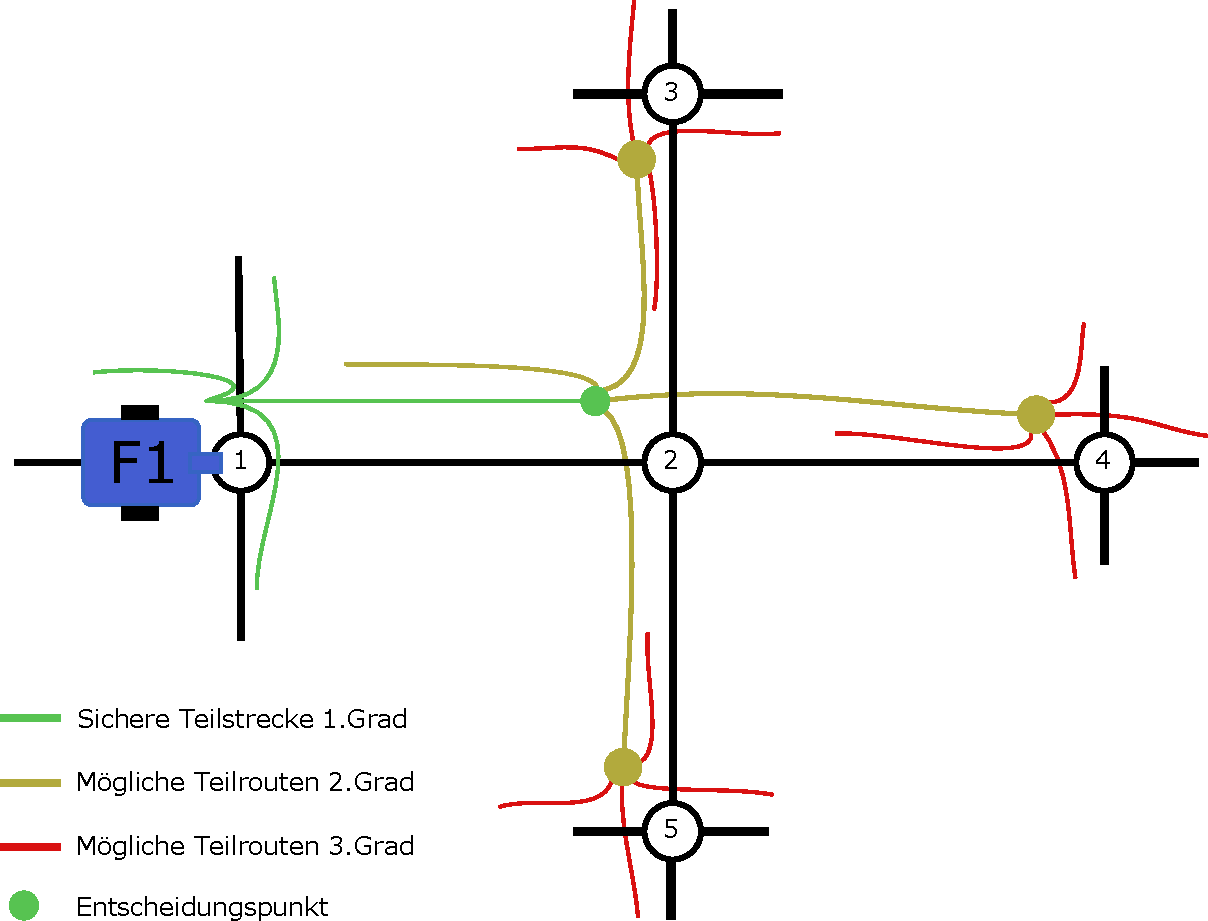
\includegraphics[scale=0.7]{/Bilder/JustificationEinstufigPDF}
			\vspace{0.2cm}
			\caption{Mögliche Teilrouten bei dreistufiger Vorhersage.}\label{Einstufig}
		\end{figure}
		
		Aus diesem Grund wurde entschieden, die dynamische Wegfindung auf der Basis einer einstufigen Positionsvorhersage zu implementieren.
		
\section{Verhinderung von Deadlock-Situationen}
	\label{Deadlock Verhindern}
	Um eine funktionsfähige Anlage zu implementieren, muss verhindert werden das sich Fahrzeuge auf der gleichen Teilstrecke entgegenkommen. Um dies zu erreichen muss der Wegberechnungsvorgang so modifiziert werden, dass die in Abschnitt \ref{Zeitproblem} eingeführte einstufige Positionsvorhersage bei der Wegfindung berücksichtigt werden kann. Da die Fahrzeuge wie in Abschnitt \ref{Externe Kommunikation} beschrieben Zugriff auf die Streckenbelegungen der anderen Fahrzeuge haben\footnote{da sie den aktuellen und geplanten nächsten Knoten über die Positionsdaten mitgeteilt bekommen, der die derzeit befahrene Teilstrecke identifiziert.}, ist dies ohne weitere Informationen bereits möglich. Bei der Aktualisierung der Positionsdaten, welche von anderen Fahrzeugen erhalten werden, wird nun zusätzlich die Position diese Fahrzeugs in einer quadratischen Matrix von der Größe der Anlagentopologie festgehalten. Diese Matrix stellt die in Abschnitt \ref{Coop Pathfinding} beschriebene dritte Dimension dar, jedoch mit der Begrenzung auf die Schritte $t_0$ und $t_{next}$.

	\subsection{Anpassung der Wegfindung}
		Durch die Einführung dieser Belegungsmatrix ist es nun möglich bei der Wegberechnung zu prüfen ob eine Teilstrecke der aktuellen Route durch ein anderes Fahrzeug besetzt ist. Dies ist jedoch nur sinnvoll für die jeweils nächste Verbindungsstrecke der aktuellen Teilroute, da weiter entfernte Strecken wahrscheinlich bereits wieder frei sind, bis das \ac{FTF} sie erreicht. Somit muss der Wegfindungsalgorithmus überprüfen, ob der die Verbindungsstrecke zum ersten Knoten entlang des kürzesten Pfads besetzt ist, und falls dies der Fall ist einen Pfad ohne diese Verbindungskante ermitteln. Genau genommen wird eine Route ermittelt, die den durch die Verbindungskante erreichbaren Knoten nicht direkt an zweiter Stelle enthält.	Dies wird erreicht, indem dem Wegfindungsbaustein als zusätzliches Argument die ID dieses Knotens übergeben wird. Bei der Wegberechnung wird dies durch zusätzlichen hohen Gewichtung der belegten Teilstrecke implementiert. Da die Anlage so konzipiert ist das es immer mindestens einen Alternativweg zu jedem Zielknoten gibt, wird die zusätzlich gewichtete Teilstrecke nicht verwendet\footnote{es kann zu Problemen führen, wenn die Alternativroute durch permanente Blockade gesperrt ist und somit die belegte Teilstrecke Teil des einzig möglichen Pfads ist. Dieser Fall müsste bei einer realen Anlage abgefangen werden, kann in der Modellanlage aber zunächst vernachlässigt werden.} 
		\\[4pt]
		Dies führt nun dazu, dass die Wegberechnung an jedem Knoten der aktuellen Route überprüfen muss, ob die jeweils nächste geplante Teilstrecke durch ein entgegenkommendes Fahrzeug belegt ist. Ist dies nicht der Fall so kann die vorher berechnete Route, wie in Abschnitt \ref{Anpassung Kommunikation} beschrieben, weiterhin verwendet werden. Ist das nächste Teilstück der Anlage jedoch belegt, muss der Weg unter dieser Voraussetzung neu berechnet werden. Dies entspricht der in Kapitel \ref{Betrachtete_Algorithmen} beschriebenen Mischform aus Planungs- und Ausführungsphase des A*-Algorithmus, bei dem an jedem Knoten eine Route unter Berücksichtigung der Umgebung geplant wird.
		\\ \textbf{insert graphic recalculate route here}
	
	\subsection{Kommunikation verifizierter Teilstrecken}
		\label{Anpassung Kommunikation}
		Die Möglichkeit, dass sich die als nächstes geplante Teilstrecke bei dem Erreichen eines Knotens ändern kann, hat zur Folge, dass auch die externe Kommunikation mit anderen Fahrzeugen modifiziert werden muss. Es kann nicht länger bei Erkennung einer Kreuzung durch den \ac{RFID}-Sensor parallel die Positionsdaten mit der geplanten Teilstrecke an die Wegfindungsschicht und die anderen Fahrzeuge gleichzeitig weitergeleitet werden. Dies würde dazu führen das nach einer notwendigen Neuberechnung durch die Wegfindung das Fahrzeug nicht mehr die vorher publik gemachte Teilstrecke befährt, sondern eine andere Verbindungsstrecke auf der neuen Route belegt. Dadurch würden entgegenkommende Fahrzeuge nicht wissen, das diese Strecke eigentlich bereits belegt ist.
		\\[4pt]
		Eine Möglichkeit ist, bei einer Änderung der geplanten Route die aktualisierten Positionsdaten erneut zu senden. Dies erhöht aber die Kommunikationslast und ist deshalb nur begrenzt sinnvoll. Als andere  Lösung wurden interne von der externen Kommunikation getrennt und zeitlich gestaffelt. Das aktualisierte Kommunikationsmodell sieht vor, das bei der Erkennung des Knotens zunächst nur die Wegfindung die geplante nächste Teilstrecke erhält. Diese verifiziert die Route und sendet in jedem Fall eine aktualisierte Route an die Fahrzeugsteuerung zurück. Diese besteht entweder aus dem Teil der noch gültigen Route, der vom aktuellen Knoten zum Zielknoten führt, oder aus der neu berechneten Ausweichroute. \textbf{insert graphics for both options here.}
		\\[4pt]
		Hat die Fahrzeugsteuerung eine Route von der Wegfindung erhalten, so teilt sie die aktualisierte nächste Teilstrecke den anderen Fahrzeugen mit. Erhält die Fahrzeugsteuerung nicht sofort eine Route\footnote{auch nicht die aktualisierte alte Route.}, so bewegt sie sich langsam weiter auf die Kreuzung zu, bis der Zeitpunkt erreicht ist, an dem die letzte Möglichkeit besteht die Route noch zu ändern. Dies ist der Zeitpunkt an dem sich das Fahrzeug genau auf der Mitte der Kreuzung befindet\footnote{da sich die Fahrzeuge auf der Stelle drehen, muss sich die mittlere Radachse genau auf der Kreuzung befinden.}. Hat das Fahrzeug bis zu diesem Zeitpunkt noch keine Rückmeldung von der Wegfindungsschicht erhalten, so bleibt es auf der Kreuzung stehen und wartet auf die Wegfindung. Die Wahrscheinlichkeit ist in diesem Fall hoch, dass die Verzögerung durch eine Belegung des nächsten Streckenabschnitts durch ein anderes Fahrzeug verursacht wurde, die eine Neuberechnung der Route mit sich bringt. Erst wenn eine Route empfangen wurde, setzt sich das Fahrzeug wieder in Bewegung.
		
		\begin{figure}[h]
			\centering
			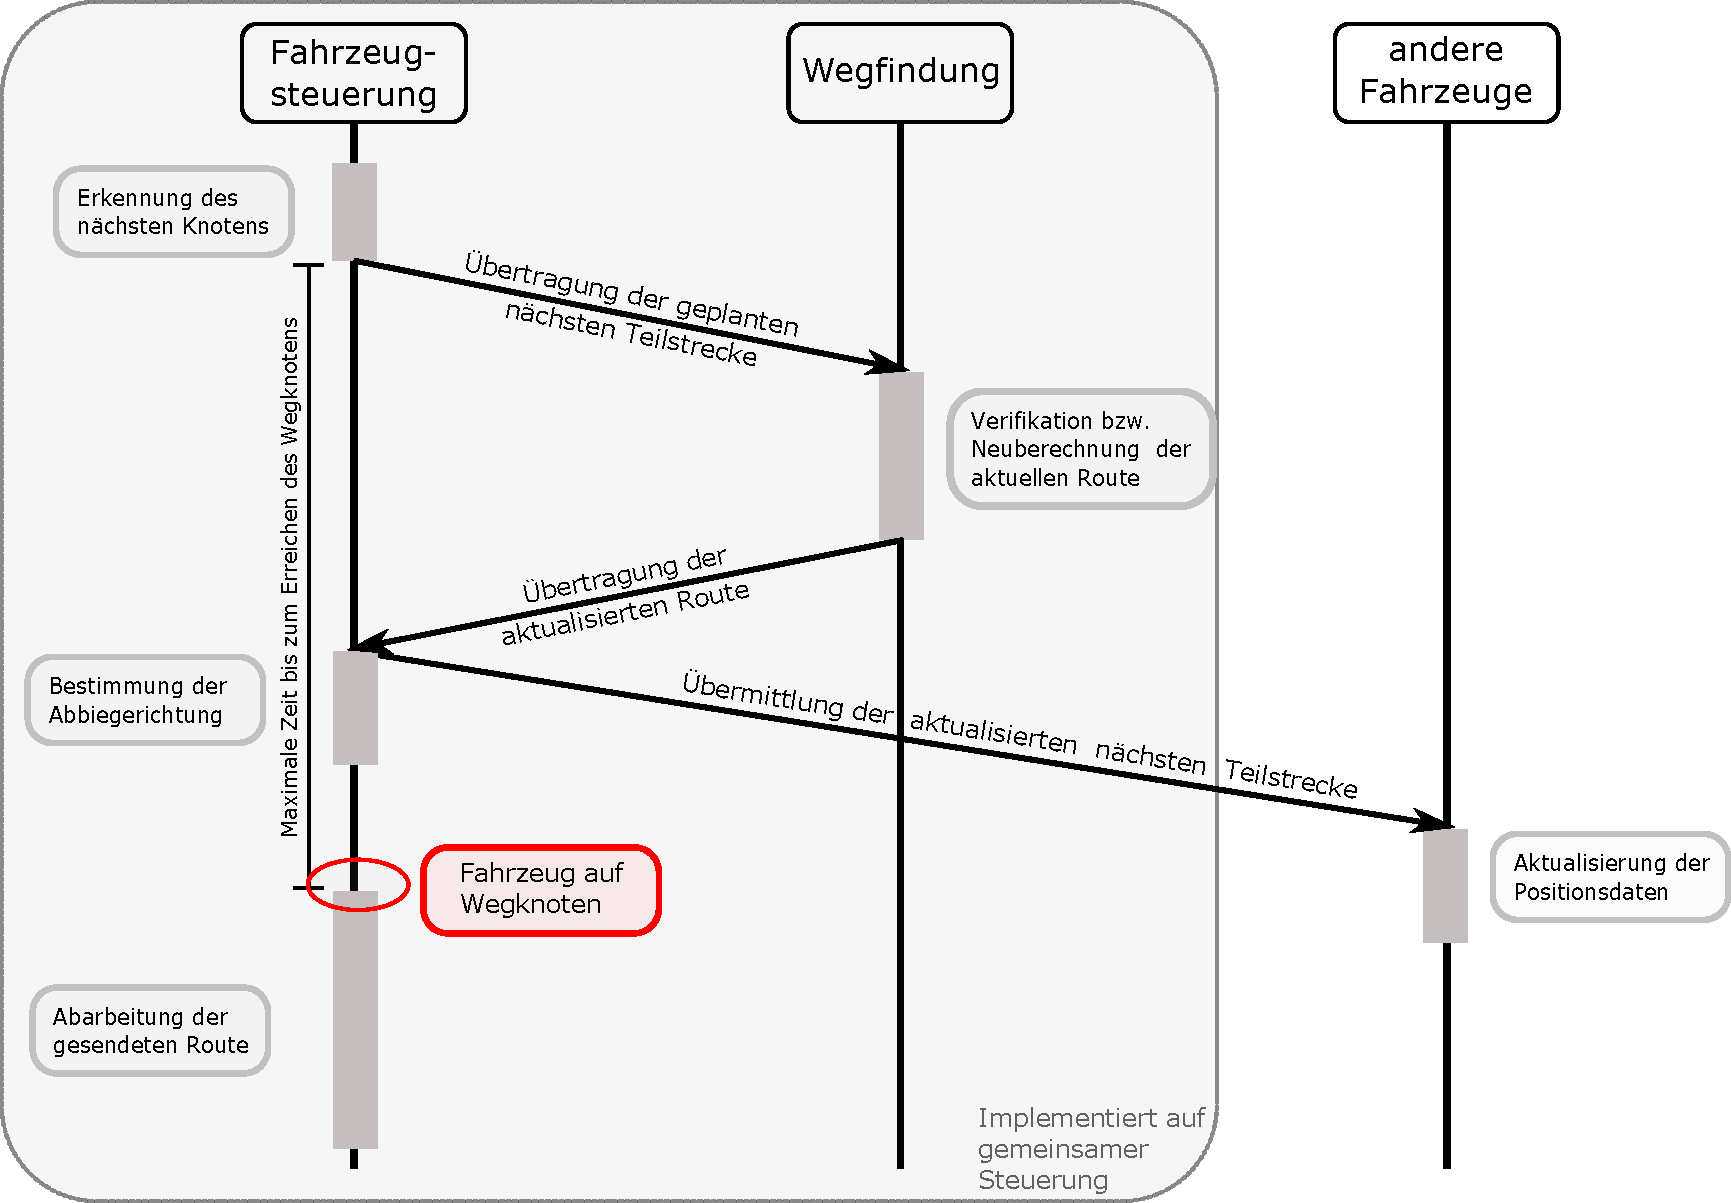
\includegraphics[scale=0.5]{/Bilder/SequenzDiagrammKommunikationPDF}
			\vspace{0.2cm}
			\caption{Sequenzdiagramm des Übertragungsvorgangs aktualisierter Teilrouten.}
		\end{figure}
		
		Um einen reibungslosen Ablauf der Anlage garantieren zu können, ist es somit wichtig, das die Neuberechnung der Route möglichst schnell ausgeführt wird. Aus diesem Grund wurde in Kapitel \ref{Implementierung} ein so hoher Wert auf die Effizienz der Implementierung der Algorithmen gelegt, um einen Halt an der Kreuzung zu vermeiden.
		
\section{Erreichte Dynamik}
	
	Mithilfe der in diesem Kapitel beschriebenen Methoden zur Kommunikation und den Änderungen an dem Ablauf der Wegfindung lässt sich ein gewisses Maß an Dynamik erreichen. Die einzelnen Fahrzeuge können auf andere Anlagenteilnehmer Rücksicht nehmen und durch die von ihnen empfangenen Informationen eine verbesserte Wegfindung durchführen. Aufgrund der vielen variablen Faktoren der realisierten Anlage lässt sich die Route aber immer nur bis zu einem bestimmten Grad vorausplanen und muss deshalb an jedem Knoten verifiziert werden. Da bei der Implementierung der Wegfindung jedoch ein besonderes Augenmerk auf die Effizienz der verwendeten Algorithmen gelegt wurde, kommt es in der Praxis nie zu einem Halt an Kreuzungen, da die aktualisierte Route immer vor dem Erreichen der Kreuzung an die Fahrzeugsteuerung übermittelt wird. Auch die in Abschnitt \ref{zyklische Auftrennung} erwähnte Erhöhung der Berechnungsdauer durch die eingeschobene Bearbeitung der anderen Schichten-\ac{OB}s hatte nur geringen Einfluss auf die Einhaltung des gegebenen Berechnungszeitrahmens.
